\section{Testberichte}
\subsection{Ballmaschine}
%\begin{figure}[h!]
	%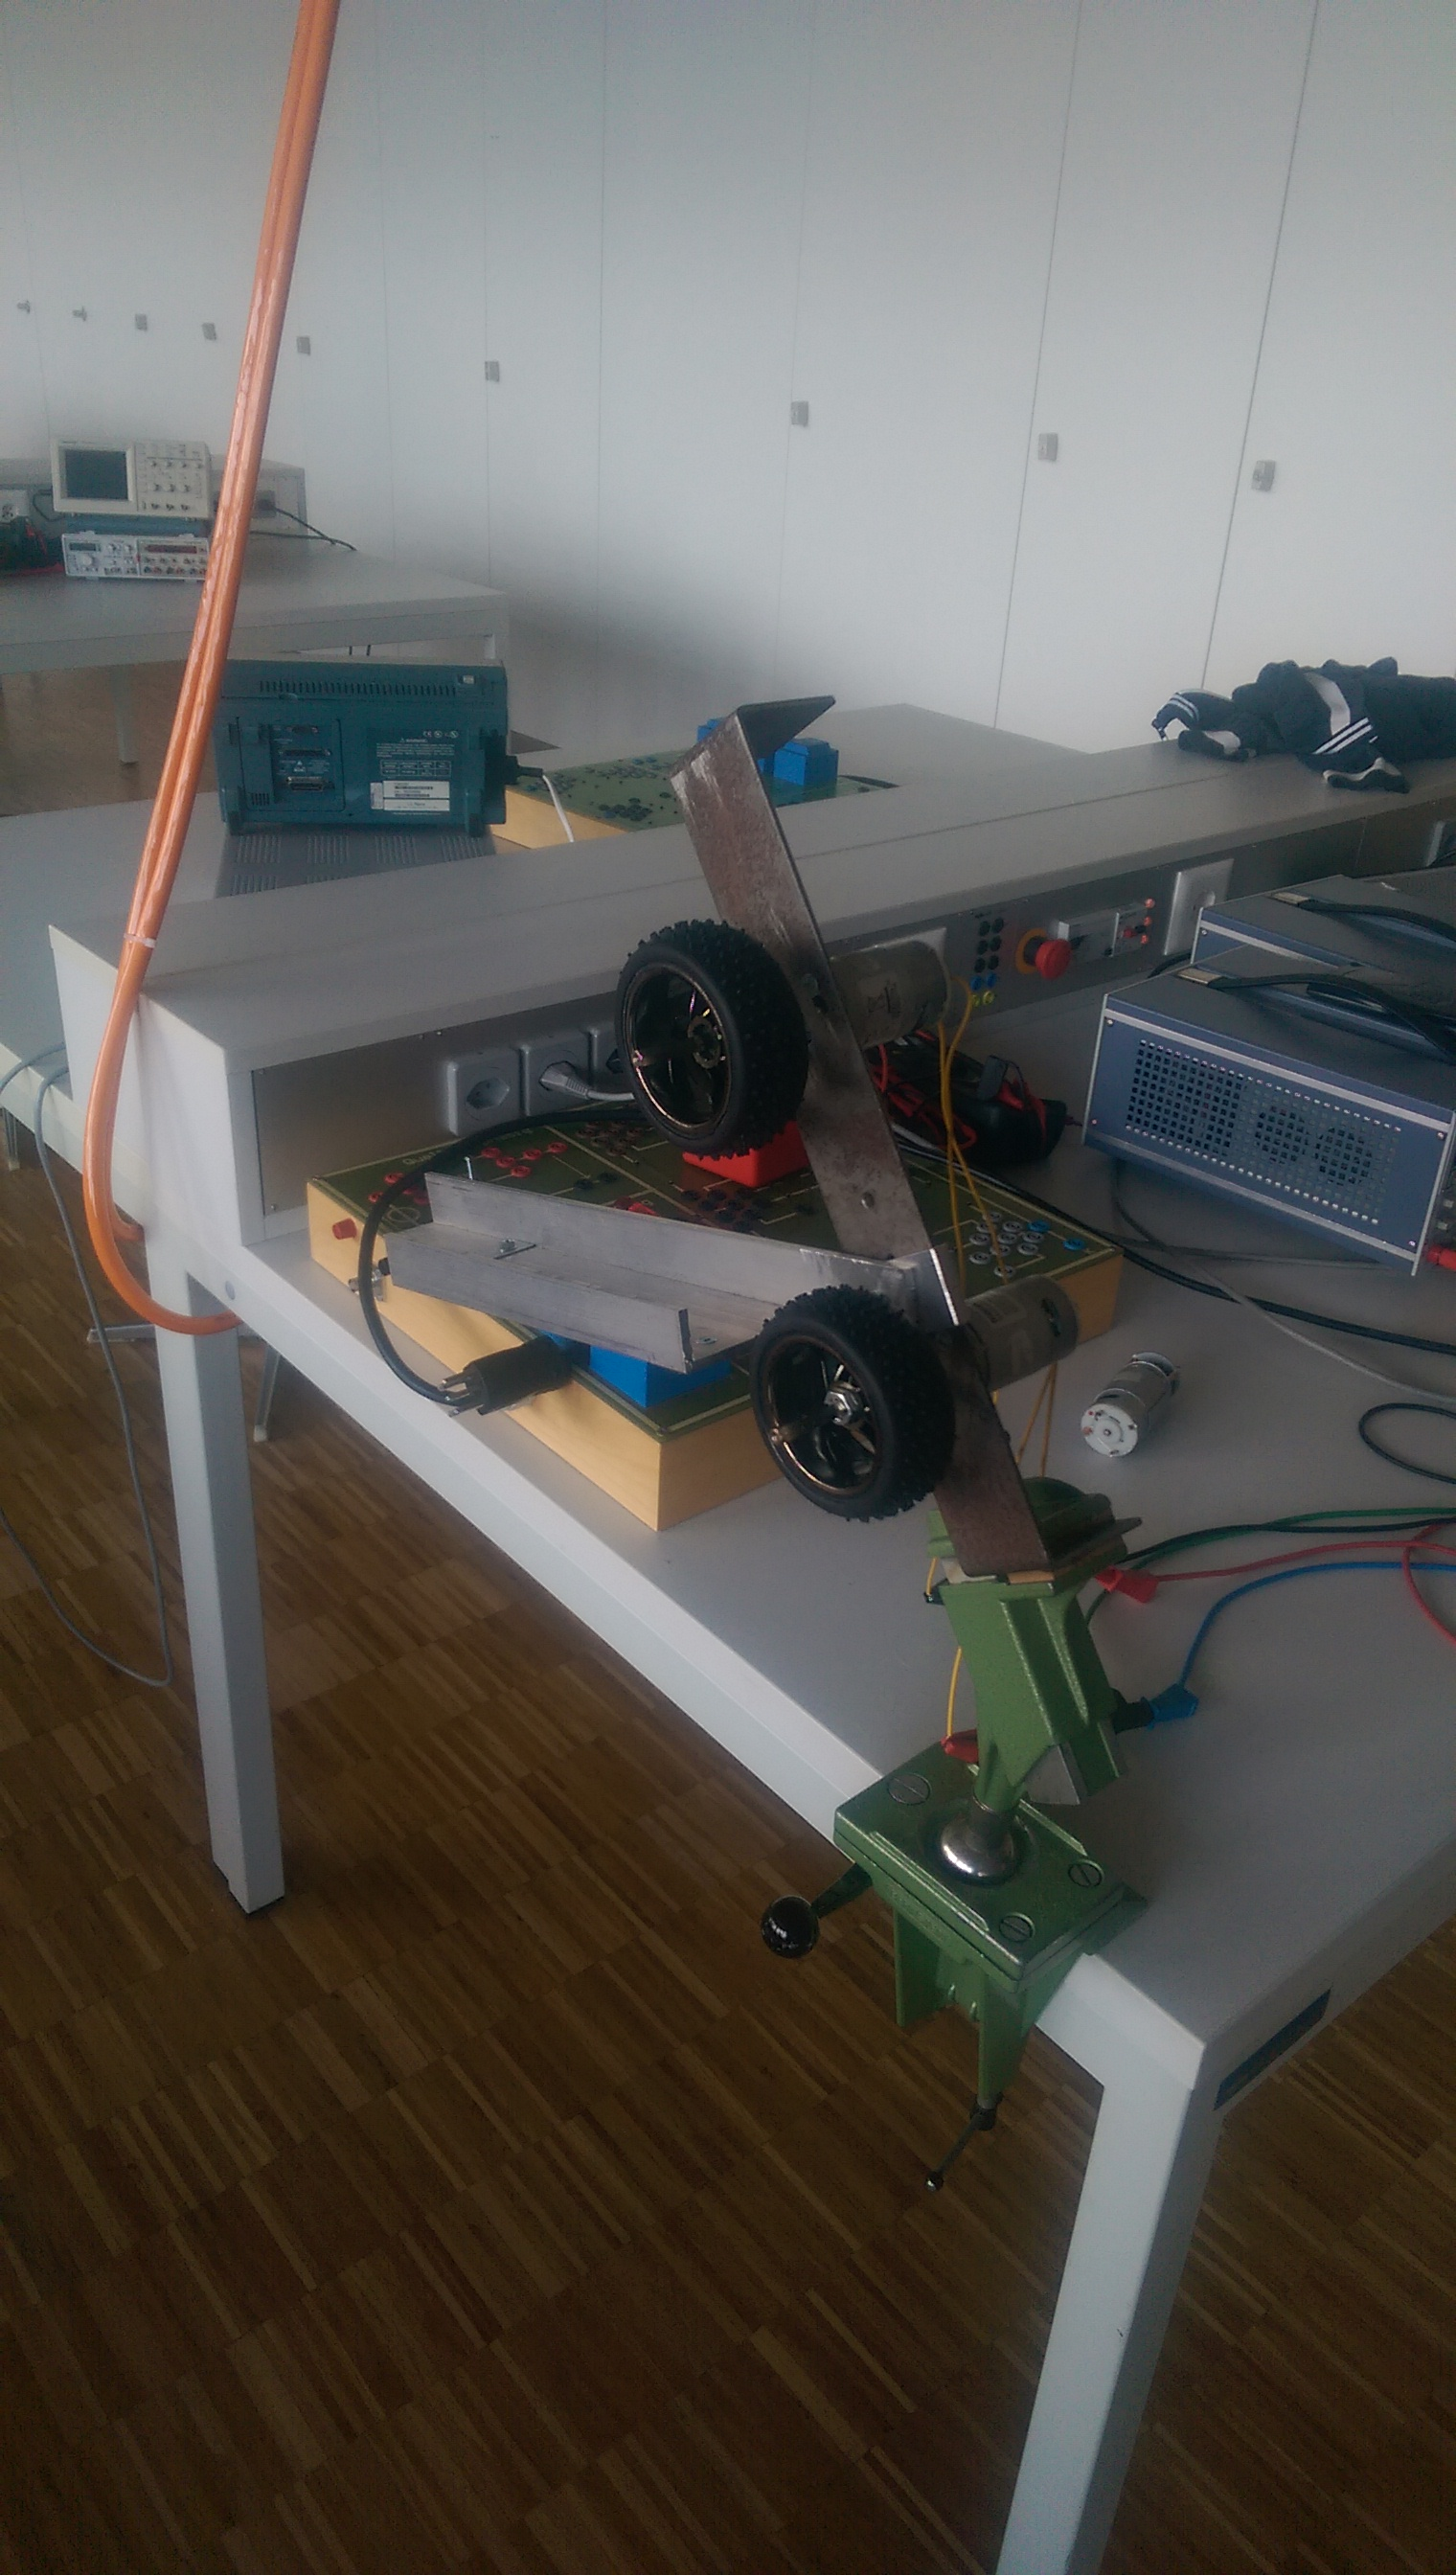
\includegraphics[scale=0.75]{Funktionstests/Bilder/Ballmaschine_Drehzahl1.jpg}
	%\centering
	%\caption{Ballmaschine_Drehzahl1} 
%\label{abb:Ballmaschine_Drehzahl1}
%\end{figure}	
Typ: Ballmaschine\\ 
Datum: 18.10.2014   \\
Ort: Labor \\
Tester: Gruppe 32 \\
Ziel des Testes:  Das Ziel dieses Testes bestand darin, den gebauten Prototyp (Ballmaschine) 
auf die Genauigkeit und Wurfweite zu testen. Erkenntnisse über die 
Drehzahl der Räder zu eruieren. Die erforderliche Stromstärke unter realen 
Bedingungen testen.  \\
Fazit/ 
Verbesserungsvorschlag: \\
Die Wurfmaschine kann mit einigen Verbesserungen sehr gute und genaue 
„Schüsse“ erzielen.  \\
Zu verbessern: 
-Stabilere Achsen  \\
-genauere und gleichmässige Zuführung der Bälle. \\
-einstellbares Grundgerüst \\
Ziel erreicht: Ja